\documentclass[11pt]{scrartcl}
\usepackage[scale=1.5]{ccicons}
\usepackage[notextcomp]{kpfonts} 
\usepackage[margin=1.0in]{geometry}
\usepackage{amsthm,amssymb,amsmath}
\usepackage{graphicx}
\usepackage{enumitem}
\usepackage{bm}
\usepackage{tabu}
\usepackage{mathtools}
\usepackage{tikz}
\usepackage{tikz-3dplot}
\usepackage{xcolor}
\usepackage{colortbl}
\usepackage{wasysym}
\usepackage{wrapfig}
\usepackage{tabularx}


\newcolumntype{C}{>{\raggedright\arraybackslash $}X<{$}}



\usepackage{color}
\definecolor{darkblue}{rgb}{0, 0, .6}
\definecolor{grey}{rgb}{.7, .7, .7}
\usepackage[breaklinks]{hyperref}
\hypersetup{
	colorlinks=true,
	linkcolor=darkblue,
	anchorcolor=darkblue,
	citecolor=darkblue,
	pagecolor=darkblue,
	urlcolor=darkblue,
	pdftitle={},
	pdfauthor={}
}
\usepackage{fancyhdr}
\thispagestyle{fancy}
\lhead{}
\chead{Math 107 Section 001 Laird}
\rhead{}
%\lfoot{}%\scriptsize This work is licensed under the \href{http://creativecommons.org/licenses/by-sa/3.0/us/}{Creative Commons Attribution-Share Alike 3.0 License}.} 
%\cfoot{}
%\rfoot{\ccbysa}
\renewcommand{\headrulewidth}{.4pt}
%\renewcommand{\footrulewidth}{.4pt}

\theoremstyle{definition}
\newtheorem{theorem}{Theorem}
\newtheorem*{theorem*}{Theorem}
\newtheorem{acknowledgement}[theorem]{Acknowledgement}
\newtheorem{algorithm}[theorem]{Algorithm}
\newtheorem{axiom}[theorem]{Axiom}
\newtheorem{case}[theorem]{Case}
\newtheorem{claim}[theorem]{Claim}
\newtheorem*{claim*}{Claim}
\newtheorem{conclusion}[theorem]{Conclusion}
\newtheorem{condition}[theorem]{Condition}
\newtheorem{conjecture}[theorem]{Conjecture}
\newtheorem{corollary}[theorem]{Corollary}
\newtheorem{criterion}[theorem]{Criterion}
\newtheorem{definition}[theorem]{Definition}
\newtheorem{example}[theorem]{Example}
\newtheorem{exercise}[theorem]{Exercise}
\newtheorem{journal}[theorem]{Journal}
\newtheorem{lemma}[theorem]{Lemma}
\newtheorem{notation}[theorem]{Notation}
\newtheorem{problem}[theorem]{Problem}
\newtheorem*{problem*}{Problem}
\newtheorem{proposition}[theorem]{Proposition}
\newtheorem{remark}[theorem]{Remark}
%\newtheorem{solution}[theorem]{Solution}
\newtheorem{summary}[theorem]{Summary}
\newtheorem{skeleton}[theorem]{Skeleton Proof}
\newtheorem{activity}[theorem]{Activity}
\newtheorem{intuitivedef}[theorem]{Intuitive Definition}

\DeclareMathOperator{\spn}{span}
\DeclareMathOperator{\Char}{Characteristic}
\DeclareMathOperator{\Aut}{Aut}
\DeclareMathOperator{\stab}{Stab}
\DeclareMathOperator{\Stab}{Stab}
\DeclareMathOperator{\orb}{\mathcal{O}}
\DeclareMathOperator{\lcm}{lcm}
\DeclareMathOperator{\gl}{GL}
\DeclareMathOperator{\Ker}{Ker}
\DeclareMathOperator{\Z}{\mathbb{Z}}
\DeclareMathOperator{\C}{\mathbb{C}}
\DeclareMathOperator{\R}{\mathbb{R}}
\DeclareMathOperator{\N}{\mathbb{N}}
\DeclareMathOperator{\Q}{\mathbb{Q}}
\DeclareMathOperator{\A}{\mathbb{A}}
\DeclareMathOperator{\Gal}{Gal}
\DeclareMathOperator{\PS}{\mathcal{P}}
\DeclareMathOperator{\acc}{acc}
\DeclareMathOperator{\mstar}{\mu^\ast}
\DeclareMathOperator{\M}{\mathcal{M}}
\DeclareMathOperator{\el}{\mathcal{L}}
\DeclareMathOperator{\dm}{d\mu}


\newenvironment{solution}{\begin{proof}[Solution]}{\end{proof}}
\newcommand{\comment}[1]{%
  \text{\phantom{(#1)}} \tag{#1}
}

\pagenumbering{gobble}

%Useful for cut and paste
%\begin{enumerate}[label=\rm{(\alph*)}]

\begin{document}

\newpage
\thispagestyle{fancy}

%\noindent
%\textit{Directions: Work individually on the following three questions. When you are finished come up front and have one of the instructors of the course review your answers to get your seating assignment for the day. No calculators are allowed for this activity.}
%
%\begin{problem}
%	Graph the equation $y=-\frac{3}{2}x+2$ on the axes below.
%	\begin{center}
%		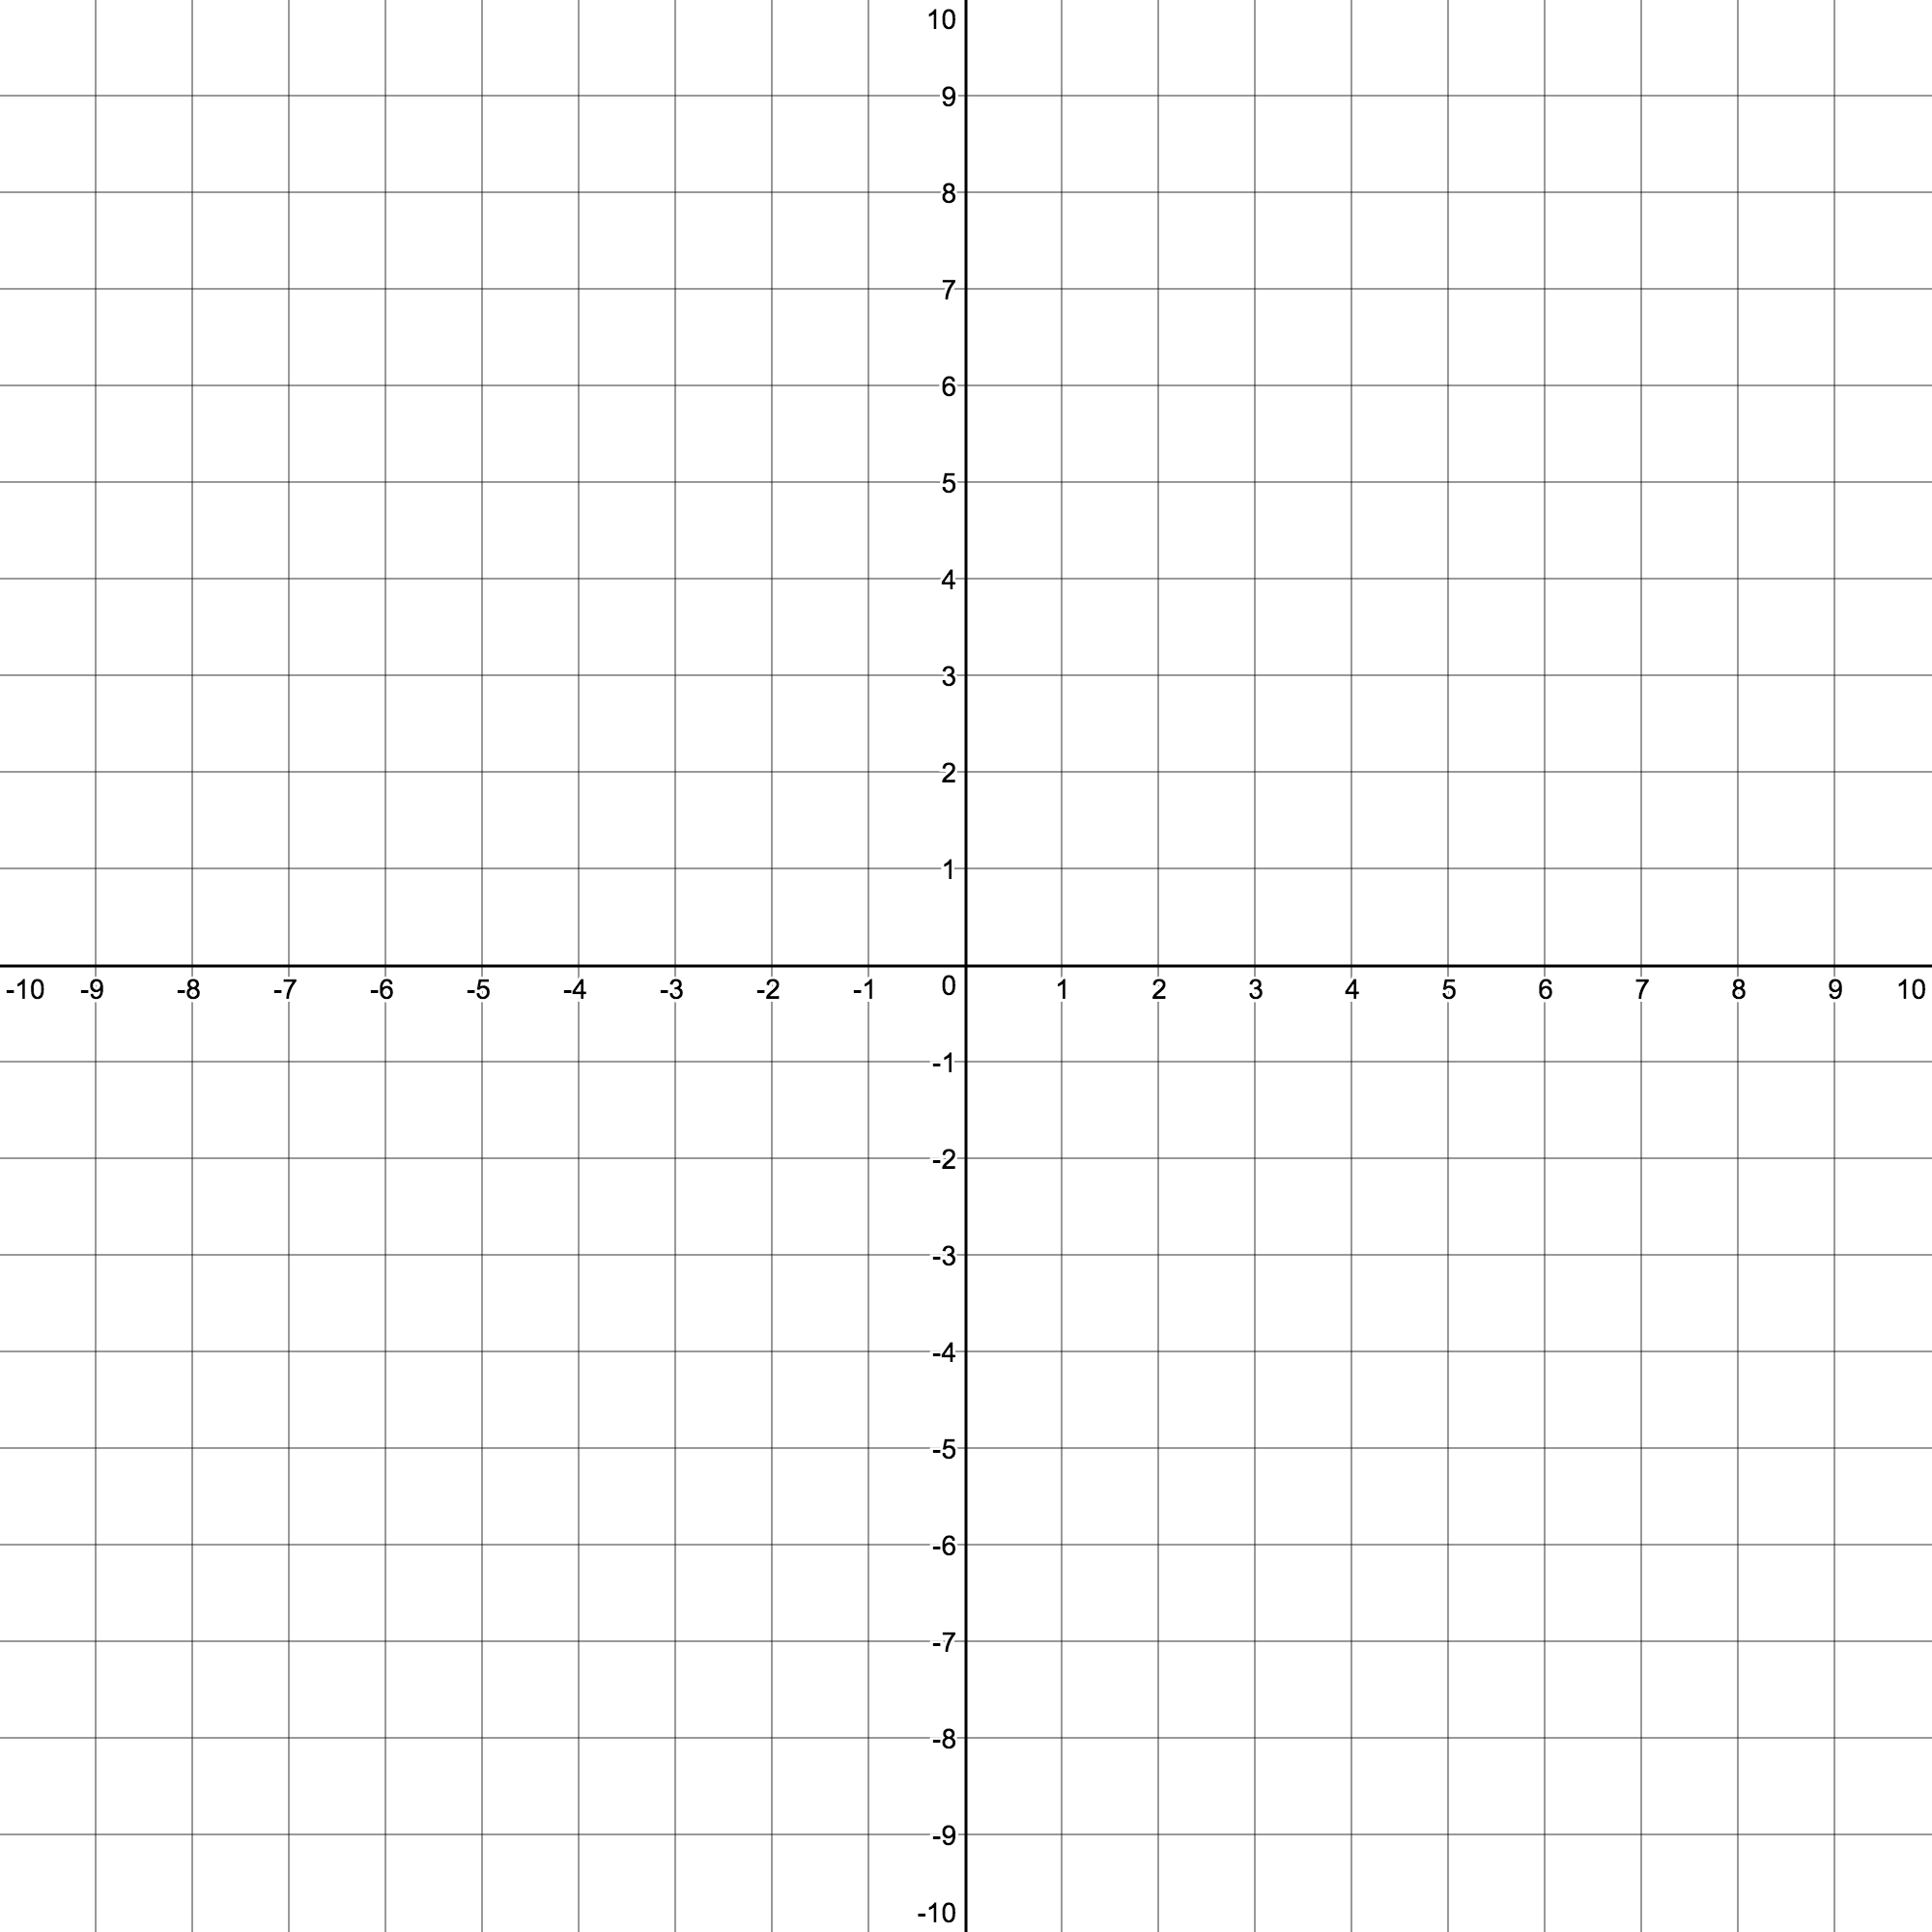
\includegraphics[scale=0.15]{grid}
%	\end{center}
%	
%	\noindent
%	Is the point $(2,-1)$ a solution to the equation?\\[3cm]
%\end{problem}
%
%\begin{problem}
%	Find all points for which -1 is a solution to the equation $y=-\frac{5}{6}x+7$. \\[3cm]
%\end{problem}
%
%\begin{problem}
%	Write an equation for the line that passes through the points $(7,12)$ and $(1,4)$.
%\end{problem}

%\noindent
%\section*{Notes:}
%\textbf{The equation for a line is given by:} \\[1cm]
%
%\noindent
%\textbf{This is called \underline{\hspace{5cm}} where $m$ is the \underline{\hspace{5cm}} and\\[2mm] $b$ is the \underline{\hspace{5cm}}.}\\[2.5cm]
%
%\subsection*{Slope}
%\textbf{The slope of a line is also known as:}
%\begin{itemize}
%	\item 
%	\item 
%	\item 
%\end{itemize}
%
%\vspace{4mm}
%
%\noindent
%\textbf{We calculate slope using the following equation:}\\[2.5cm]
%
%\subsection*{Solving for points}
%\textbf{When we are given an $x$-value and we are asked to find $y$, we do the following:}\\[3cm]
%
%\noindent
%\begin{example}
%	Consider the equation $y=3x-5$. Find $y$ when $x$ is $4$.
%\end{example}
%
%\newpage
%
%\noindent
%\textbf{When we are given a $y$-value and we are asked to find $x$, we do the following:}\\[2.5cm]
%
%\noindent
%\begin{example}
%	Consider the equation $y=3x-5$. Find $x$ when $y$ is 13.	
%\end{example}
%
%
%\noindent
%\subsection*{Graphing}
%\textbf{Given an equation we graph it in the following way:}\\[2.5cm]
%
%\begin{example}
%	Graph the equation $y=3x-4$.
%	\begin{center}
%		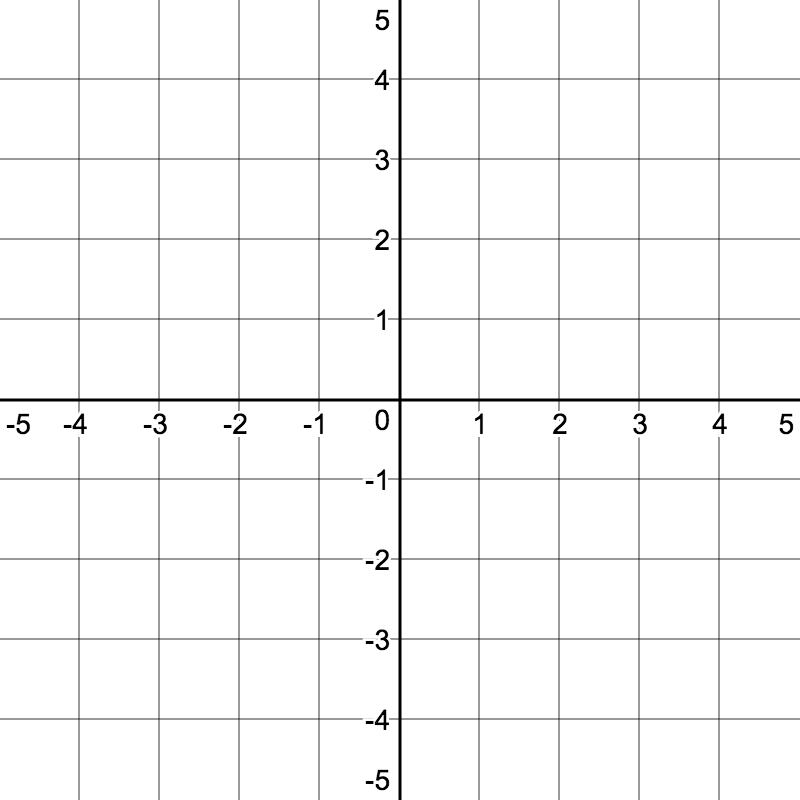
\includegraphics[scale=0.15]{5x5grid}
%	\end{center}
%\end{example}
%
%\vspace{2mm}
%
%\noindent
%\textbf{Given the slope and a point we graph the line in the following way:}\\[2.5cm]
%
%\begin{example}
%	Graph the line that has a slope of -2 and goes through the point $(2,3)$.
%	\begin{center}
%		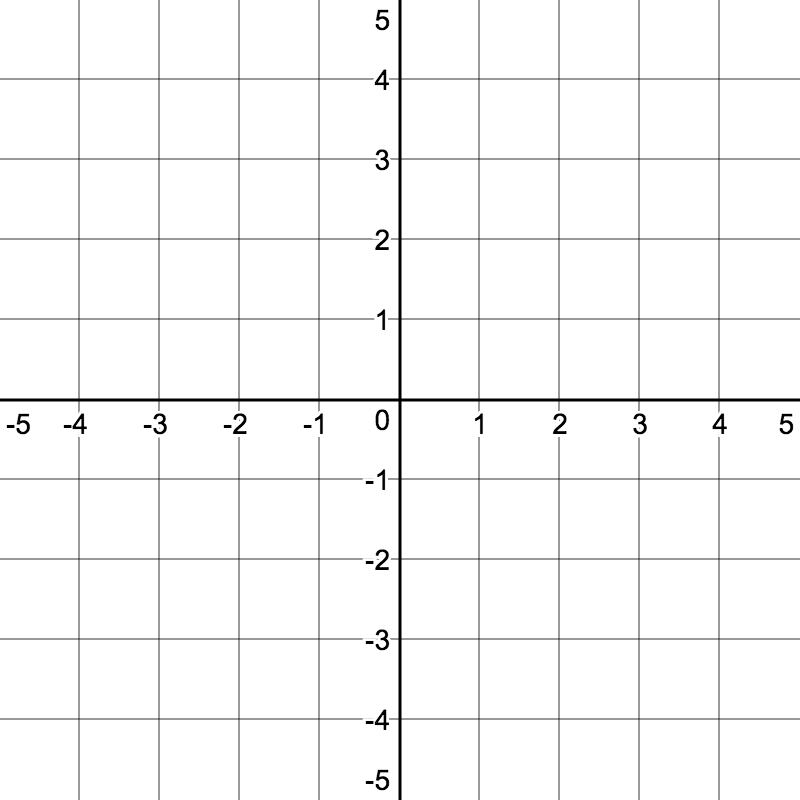
\includegraphics[scale=0.15]{5x5grid}
%	\end{center}
%\end{example}
%
%\newpage
%\subsection*{Practice Problems}
%\begin{problem}
%	The number of Americans without health insurance was 46.7 million in 2010, and it increased by about 1.04 million per year until 2013. Let $n$ be the number in millions of Americans without health insurance at $t$ years since 2010.
%	\begin{itemize}
%		\item Identify the slope of the model. What does it mean in this situation?
%		\item Identify the y-intercept. What does it mean in this situation?
%		\item Write an equation to model this situation.
%		\item Estimate when 49 million Americans did not have health insurance.
%		\item How many millions of people were without health insurance in 2012?
%	\end{itemize}
%\end{problem}
%
%\vspace{4mm}
%
%%\begin{problem}
%%	The minimum salary for a hockey player in the National Hockey League was \$500 thousand in 2010, and it increased by about \$14 thousand per year until 2015. Let $s$ be the minimum salary (in thousands of dollars) at $t$ years since 2010.
%%	\begin{itemize}
%%		\item Identify the rate of change of this situation. What does this mean in this situation?
%%		\item Identify the $y$-intercept for creating a linear model. What does it mean in this situation?
%%		\item Write an equation to model this situation.
%%		\item What was the minimum salary in 2015?
%%		\item When was the minimum salary \$550 thousand?
%%	\end{itemize}
%%\end{problem}
%
%\vspace{4mm}
%
%\begin{problem}
%	In 2010, the percentage of private-sector workers who were in a union was 6.95\%, and it decreased by about 0.25 percentage points per year until 2014.
%	\begin{itemize}
%		\item Find an equation of a model to describe the situation. Explain what your variables represent.
%		\item Estimate when the percentage of unionized workers was 6.20\%.
%		\item Estimate the percentage of private-sector workers who were \underline{not} in a union in 2014.
%	\end{itemize}
%\end{problem}
%
%\vspace{4mm}
%
%\begin{problem}
%	uberXL in Tucson charges a \$2.50 base fare, a \$2.05 booking fee and a per mile charge of \$1.65. If I paid \$18.41 for an uberXL trip, how far did I go?
%\end{problem}
%
%\vspace{4mm}
%
%\begin{problem}
%	The percentages of college freshmen whose average grade in high school was an A are shown below:
%	\begin{center}
%		\begin{tabular}{c|c}
%Year & Percent \\ \hline
%1970 & 19.6    \\
%1980 & 26.6    \\
%1985 & 28.7    \\
%1990 & 29.4    \\
%1995 & 36.1    \\
%2000 & 42.9    \\
%2005 & 46.6    \\
%2010 & 48.4   
%\end{tabular}
%	\end{center}
%Let $p$ be the percentage of college freshmen whose average grade in high school was an A at $t$ years since 1970.
%\begin{itemize}
%	\item Construct a scatterplot.
%	\item Describe the four characteristics of the association. (make sure to include $r$)
%	\item A model of the situation is $p=0.76t_18.06$. Graph the model on the scatterplot (try to do this by hand!). 
%	\item Does it come close to the data points?
%	\item Estimate when 44\% of all college freshmen earned an average grade of A in high school.
%	\item Using the linear model predict the percentage of college freshmen that earned an average grade A in high school this year.
%\end{itemize}		
%\end{problem}

%\noindent
%\begin{problem}
%	Consider the following two equations of lines:
%	\[y=-3x-5 \hspace{2.5cm} y=\frac{1}{3}x+\frac{5}{3}\]
%	\begin{enumerate}[label=\alph*)]
%		\item Find 4 solutions to the two linear equations.
%		\item Carefully graph the equations on the same set of axes.
%		\item Find the intersection points of the lines and write them as an ordered pair (by using your graph)
%		\item Use your graph to solve this equation $\frac{1}{3}x+\frac{5}{3}=2$.
%		\item Solve the following equation by rules of algebra. Carefully write out each step $\frac{1}{3}x+\frac{5}{3}=2$.
%		\item Explain the relation between solving the equation and finding the answer on a graph.
%		\item Repeat 4--6 for the equation $-3x-5=\frac{1}{3}x+{5}{3}$
%		\item Discuss how you could check your answers, then check them!
%	\end{enumerate}	
%\end{problem}
%
%\begin{problem}
%	The number of Americans without health insurance was 46.7 million in 2010, and it increased by about 1.04 million per year until 2013. Let $n$ be the number in millions of Americans without health insurance at $t$ years since 2010.
%	\begin{enumerate}[label=\alph*)]
%		\item Identify the slope of the model. What does it mean in this situation?
%		\item Identify the y-intercept. What does it mean in this situation?
%		\item Write an equation to model this situation.
%		\item Estimate when 49 million Americans did not have health insurance.
%		\item How many millions of people were without health insurance in 2012?
%	\end{enumerate}
%\end{problem}
%
%\vspace{4mm}
%
%\begin{problem}
%	The minimum salary for a hockey player in the National Hockey League was \$500 thousand in 2010, and it increased by about \$14 thousand per year until 2015. Let $s$ be the minimum salary (in thousands of dollars) at $t$ years since 2010.
%	\begin{enumerate}[label=\alph*)]
%		\item Identify the rate of change of this situation. What does this mean in this situation?
%		\item Identify the $y$-intercept for creating a linear model. What does it mean in this situation?
%		\item Write an equation to model this situation.
%		\item What was the minimum salary in 2015?
%		\item When was the minimum salary \$550 thousand?
%	\end{enumerate}
%\end{problem}
%
%\vspace{4mm}
%
%\begin{problem}
%	In 2010, the percentage of private-sector workers who were in a union was 6.95\%, and it decreased by about 0.25 percentage points per year until 2014.
%	\begin{enumerate}[label=\alph*)]
%		\item Find an equation of a model to describe the situation. Explain what your variables represent.
%		\item Estimate when the percentage of unionized workers was 6.20\%.
%		\item Estimate the percentage of private-sector workers who were \underline{not} in a union in 2014.
%	\end{enumerate}
%\end{problem}
%
%\begin{problem}
%	uberXL in Tucson charges a \$2.50 base fare, a \$2.05 booking fee and a per mile charge of \$1.65. If I paid \$18.41 for an uberXL trip, how far did I go?
%\end{problem}
%
%\vspace{4mm}
%
%\begin{problem}
%	The percentages of college freshmen whose average grade in high school was an A are shown below:
%	\begin{center}
%		\begin{tabular}{c|c}
%Year & Percent \\ \hline
%1970 & 19.6    \\
%1980 & 26.6    \\
%1985 & 28.7    \\
%1990 & 29.4    \\
%1995 & 36.1    \\
%2000 & 42.9    \\
%2005 & 46.6    \\
%2010 & 48.4   
%\end{tabular}
%	\end{center}
%Let $p$ be the percentage of college freshmen whose average grade in high school was an A at $t$ years since 1970.
%\begin{enumerate}[label=\alph*)]
%	\item Construct a scatterplot.
%	\item Describe the four characteristics of the association. (make sure to include $r$)
%	\item A model of the situation is $p=0.76t_18.06$. Graph the model on the scatterplot (try to do this by hand!). 
%	\item Does it come close to the data points?
%	\item Estimate when 44\% of all college freshmen earned an average grade of A in high school.
%	\item Using the linear model predict the percentage of college freshmen that earned an average grade A in high school this year.
%\end{enumerate}		
%\end{problem}
%
%\begin{problem}
%	In 2013, the mean annual per-person consumption of butter was 5.5 pounds, up 12.2\% from 2010. What was the mean annual per person consumption of butter in 2010?
%\end{problem}
%
%\begin{problem}
%	Scientists are studying the effects of several factors on the growth of a certain species of tree. The diameter of this species of tree increases approximately 0.2 inches every six months. Scientists begin observing the trees when they are saplings, at which point they have an initial diameter of 0.3 inches. Using this information answer the following questions.
%\begin{enumerate}[label=\alph*)]
%	\item Write the general equation describing the relationship between the diameter of a given tree and the amount of time it has been observed by the scientists.
%	\item How long must scientists observe a given tree for it to grow a total diameter of 2.6 inches?
%	\item Circle all of the following statements which are consistent with the slope of the linear relationship defined above.
%	\begin{itemize}
%		\item The diameter increases 1 inch every year
%		\item In 2 years, the diameter will increase 0.8 inches
%		\item In order to see an increase in diameter of 1 inch, the scientists must observe for 2.5 years
%		\item Over the course of 18 months, the diameter will increase 0.6 inches
%		\item An increase in diameter of 0.5inches will occur in one month
%	\end{itemize}
%\end{enumerate}	
%\end{problem}

\begin{problem}
	Scientists are studying the effects of several factors on the growth of a certain species of tree. The diameter of this species of tree increases approximately 0.2 inches every six months. Scientists begin observing the trees when they are saplings, at which point they have an initial diameter of 0.3 inches. Using this information answer the following questions.
\begin{enumerate}[label=\alph*)]
	\item Write the general equation describing the relationship between the diameter of a given tree and the amount of time it has been observed by the scientists.
	\item How long must scientists observe a given tree for it to grow a total diameter of 2.6 inches?
	\item Circle all of the following statements which are consistent with the slope of the linear relationship defined above.
	\begin{itemize}
		\item The diameter increases 1 inch every year
		\item In 2 years, the diameter will increase 0.8 inches
		\item In order to see an increase in diameter of 1 inch, the scientists must observe for 2.5 years
		\item Over the course of 18 months, the diameter will increase 0.6 inches
		\item An increase in diameter of 0.5inches will occur in one month
	\end{itemize}
\end{enumerate}	
\end{problem}

\noindent
\textbf{For questions 2 through 5 complete them in the following way:}
\begin{itemize}
	\item \textbf{Write down a "ball-park estimate" of the answer, i.e. without doing any major calculations, what do you think it should be?}
	\item \textbf{ Define a variable to represent the exact answer.}
	\item \textbf{Set up an equation with the variable in it.}
	\item \textbf{Solve the equation using a calculator as necessary.}
	\item \textbf{Check your answer against your estimate and the problem, does your solution make sense?}
\end{itemize}

\begin{problem}
	In 2013, the mean annual per-person consumption of butter was 5.5 pounds, up 12.2\% from 2010. What was the mean annual per person consumption of butter in 2010?
\end{problem}

\begin{problem}
	In 2013, the sales of Monster energy drinks were \$3.1 billion, which was about 35\% of all energy drink sales. What were the total sales of all energy drinks?
\end{problem}

\begin{problem}
	In 2013, the student-teacher ration in U.S. public schools was 15.1, down 5.6\% from 2000. What was the ration in 2000?
\end{problem}

\begin{problem}
	In 2017, the cost of in-state tuition at public four-year colleges rose \$300, representing a 3.2\% increase. How much is tuition after this increase?
\end{problem}

\begin{problem}
	The number of Americans without health insurance was 46.7 million in 2010, and it increased by about 1.04 million per year until 2013. Let $n$ be the number in millions of Americans without health insurance at $t$ years since 2010.
	\begin{enumerate}[label=\alph*)]
		\item Identify the slope of the model. What does it mean in this situation?
		\item Identify the y-intercept. What does it mean in this situation?
		\item Write an equation to model this situation.
		\item Estimate when 49 million Americans did not have health insurance.
		\item How many millions of people were without health insurance in 2012?
	\end{enumerate}
\end{problem}

\vspace{4mm}

\begin{problem}
	The minimum salary for a hockey player in the National Hockey League was \$500 thousand in 2010, and it increased by about \$14 thousand per year until 2015. Let $s$ be the minimum salary (in thousands of dollars) at $t$ years since 2010.
	\begin{enumerate}[label=\alph*)]
		\item Identify the rate of change of this situation. What does this mean in this situation?
		\item Identify the $y$-intercept for creating a linear model. What does it mean in this situation?
		\item Write an equation to model this situation.
		\item What was the minimum salary in 2015?
		\item When was the minimum salary \$550 thousand?
	\end{enumerate}
\end{problem}

\vspace{4mm}

\begin{problem}
	In 2010, the percentage of private-sector workers who were in a union was 6.95\%, and it decreased by about 0.25 percentage points per year until 2014.
	\begin{enumerate}[label=\alph*)]
		\item Find an equation of a model to describe the situation. Explain what your variables represent.
		\item Estimate when the percentage of unionized workers was 6.20\%.
		\item Estimate the percentage of private-sector workers who were \underline{not} in a union in 2014.
	\end{enumerate}
\end{problem}

\begin{problem}
	uberXL in Tucson charges a \$2.50 base fare, a \$2.05 booking fee and a per mile charge of \$1.65. If I paid \$18.41 for an uberXL trip, how far did I go?
\end{problem}

\vspace{4mm}

\begin{problem}
	The percentages of college freshmen whose average grade in high school was an A are shown below:
	\begin{center}
		\begin{tabular}{c|c}
Year & Percent \\ \hline
1970 & 19.6    \\
1980 & 26.6    \\
1985 & 28.7    \\
1990 & 29.4    \\
1995 & 36.1    \\
2000 & 42.9    \\
2005 & 46.6    \\
2010 & 48.4   
\end{tabular}
	\end{center}
Let $p$ be the percentage of college freshmen whose average grade in high school was an A at $t$ years since 1970.
\begin{enumerate}[label=\alph*)]
	\item Construct a scatterplot.
	\item Describe the four characteristics of the association. (make sure to include $r$)
	\item A model of the situation is $p=0.76t_18.06$. Graph the model on the scatterplot (try to do this by hand!). 
	\item Does it come close to the data points?
	\item Estimate when 44\% of all college freshmen earned an average grade of A in high school.
	\item Using the linear model predict the percentage of college freshmen that earned an average grade A in high school this year.
\end{enumerate}		
\end{problem}









\end{document}
























